\documentclass[glossy,aspectratio=169]{beamer}
\beamertemplatenavigationsymbolsempty
\usepackage[utf8]{inputenc}
\useoutertheme{wuerzburg}
\useinnertheme[realshadow,corners=2pt,padding=2pt]{chamfered}
\usecolortheme{whale}
\usepackage[ngerman]{babel}
\usepackage{graphics, graphicx}
\usepackage{color}
\usepackage{latexsym}
\usepackage{etoolbox}
\usepackage{subfig}
\usepackage{tikz}
\PassOptionsToPackage{hyphens}{url}
\usepackage{hyperref}
\usepackage{url}
\usepackage{qrcode}
\usepackage{eurosym}

\newcommand<>{\hover}[1]{\uncover#2{%
		\begin{tikzpicture}[remember picture,overlay]%
		\draw[fill,opacity=0.4] (current page.south west)
		rectangle (current page.north east);
		\node at (current page.center) {#1};
		\end{tikzpicture}}
}

\definecolor{pblue}{rgb}{0.13,0.13,1}
\definecolor{pgreen}{rgb}{0,0.5,0}
\definecolor{pred}{rgb}{0.9,0,0}
\definecolor{pgrey}{rgb}{0.46,0.45,0.48}
\definecolor{darkgreen}{rgb}{0,0.5,0}


\title{Fachschaftsvorstellung}
\author{\textbf{fsi}}

\begin{document}
	%\maketitle
	\begin{frame}
		\centering
		
\includegraphics[width=0.8\textwidth]{pictures/fsilogo_neu.pdf}\\
		\vspace*{1cm}
		\begin{huge}
			Fachschaft? Kann man das essen?
		\end{huge}
	\end{frame}
	
	\begin{frame}{Wer sind wir?}
		\begin{figure}
			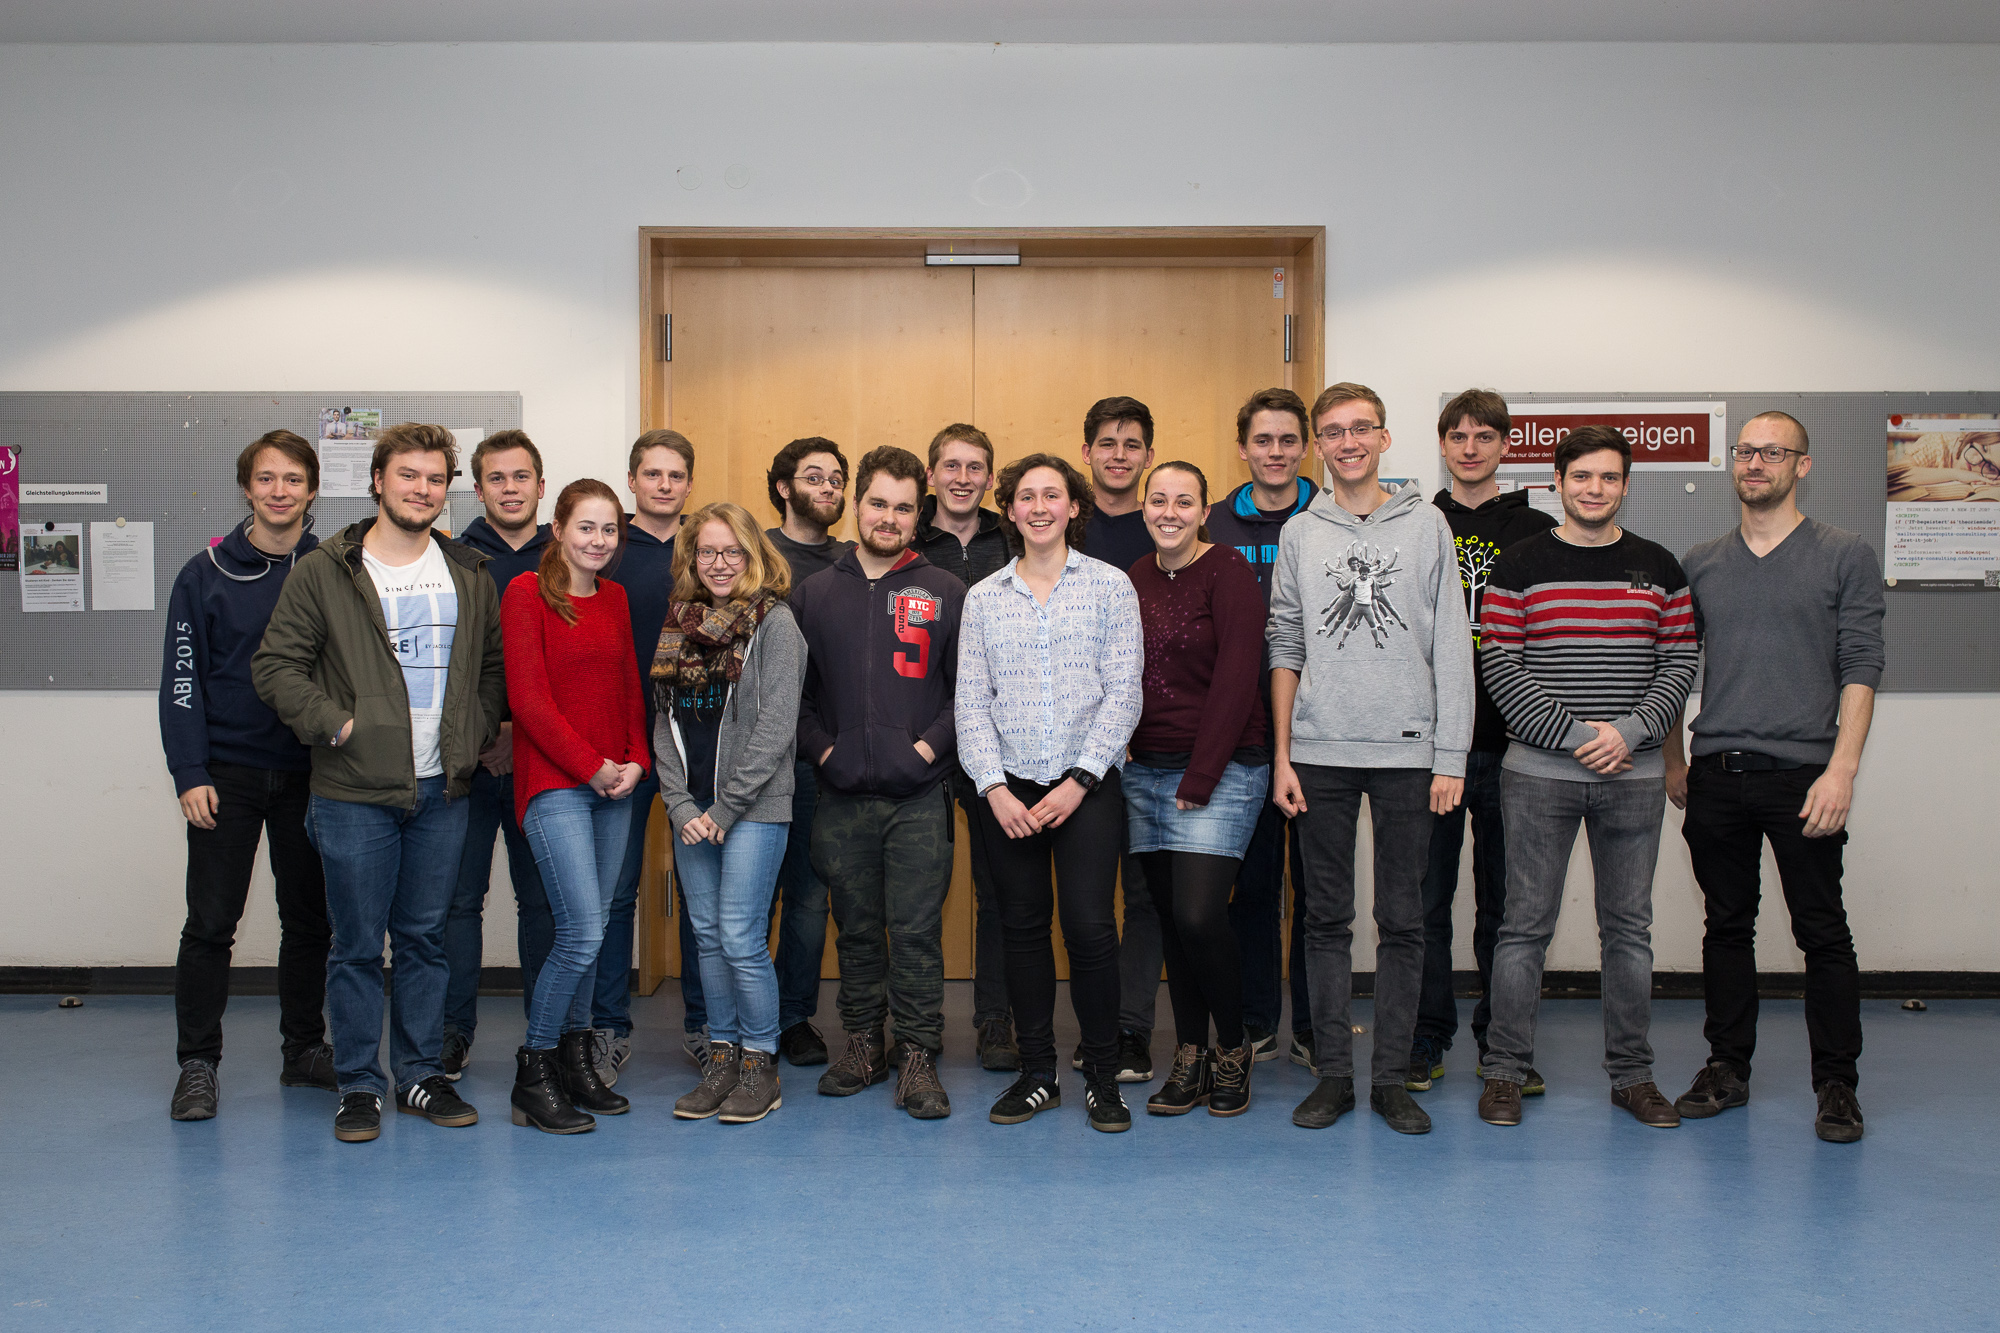
\includegraphics[height=0.9\textheight]{pictures/fachschaft_17.jpg}
		\end{figure}
	\end{frame}
	
	\begin{frame}{Was machen wir?}
		\begin{figure}
			%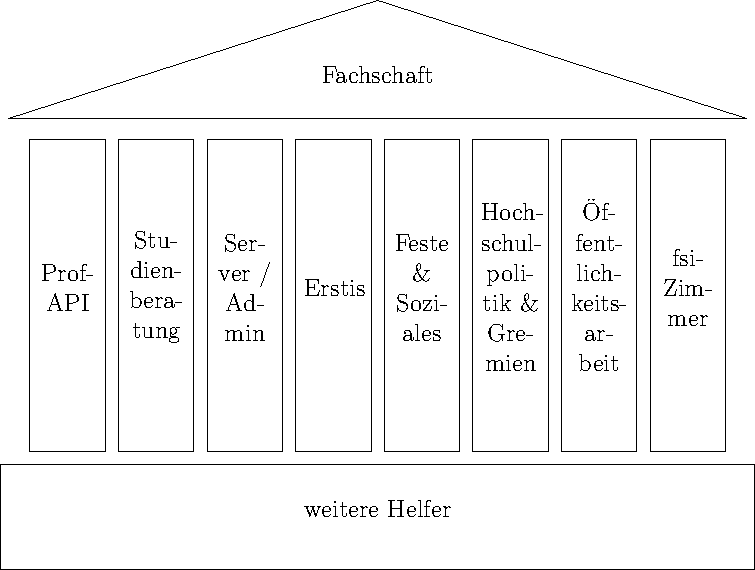
\includegraphics[width=0.9\textwidth]{pictures/selbstverstaendnis.pdf}
		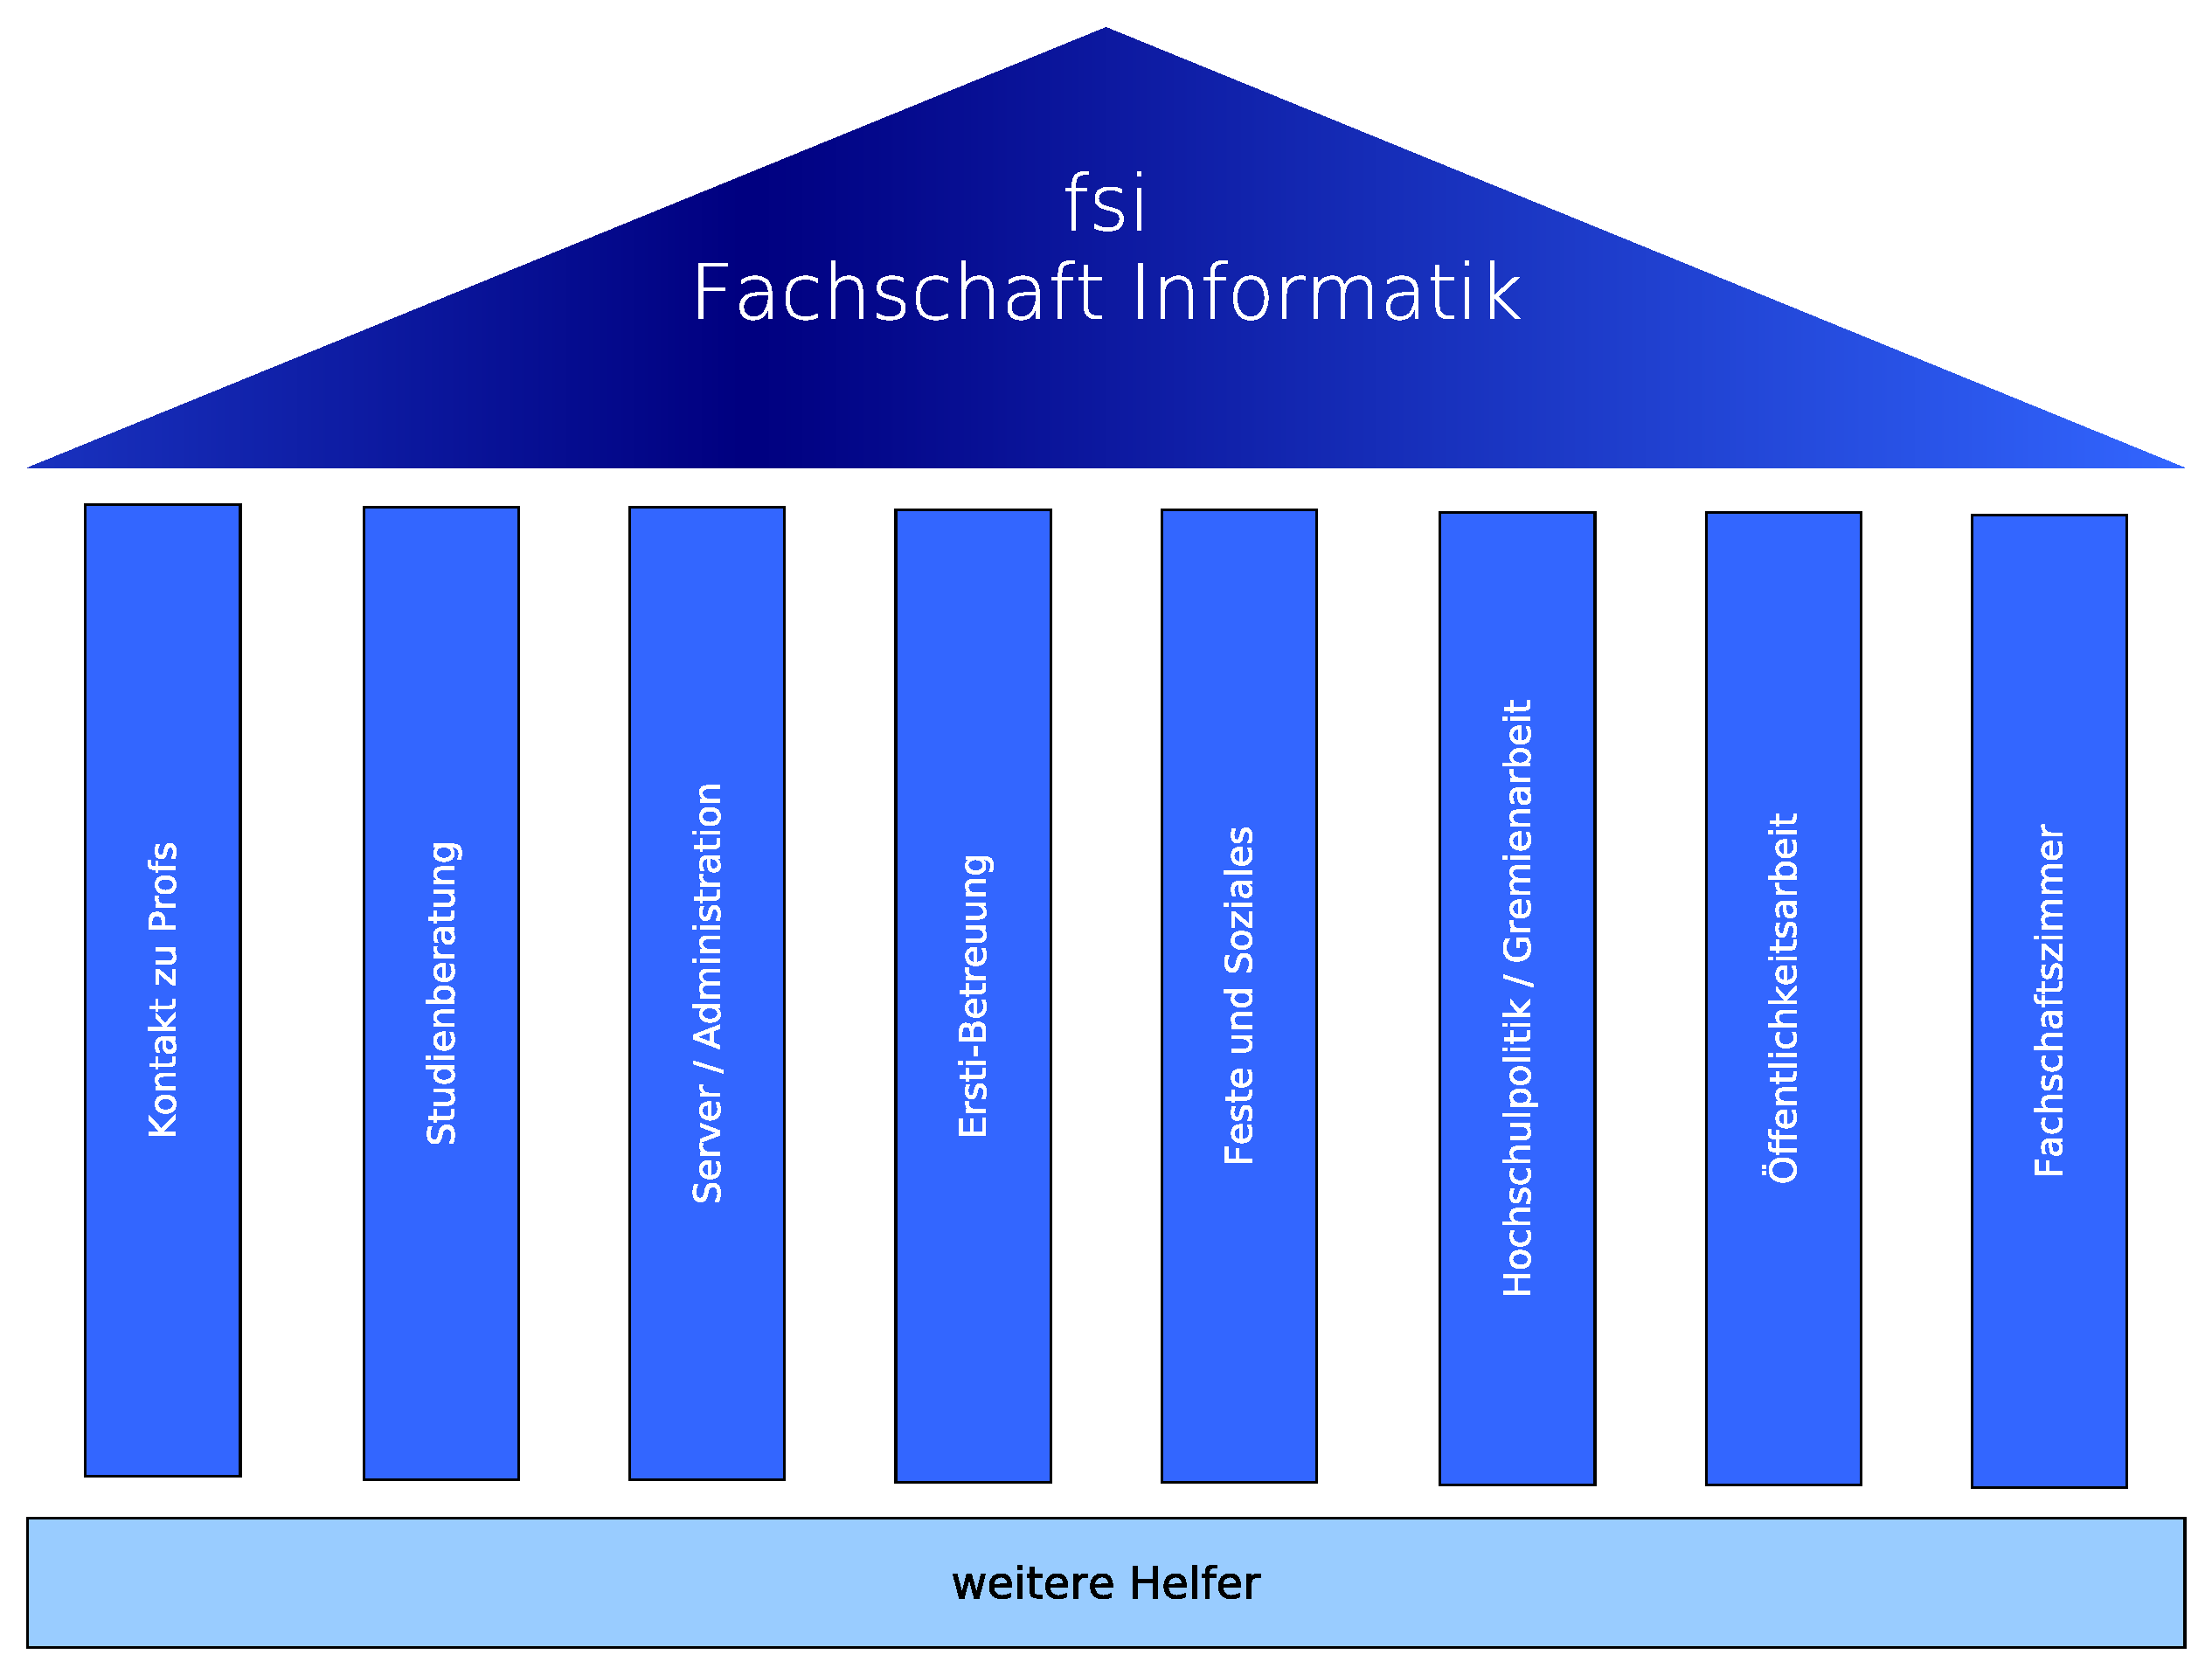
\includegraphics[height=0.8\textheight]{pictures/fsi_saeulen.pdf}
		\end{figure}
	\end{frame}
 	
	\begin{frame}{Kontakt zu Profs}
		\pause 
		\begin{itemize}[<+->]
			\item stehen in engem Kontakt mit der Professorenschaft
			\item können Probleme daher gut ansprechen
			\item (und meistens auch beheben)
			\item monatliche Treffen mit dem Fachbereich, um Problemen vorzubeugen
			\item[$\Rightarrow$] Wir brauchen euren Input!\\Also kommt zu uns, wenn ihr Probleme habt!
		\end{itemize}
	\end{frame}
	
	\begin{frame}{Studienberatung}
		\pause 
		\begin{itemize}[<+->]		
			\item \textbf{Informatik \& Bioinformatik}\quad Berater: Thomas Sachs\\
			E-Mail: studienberatung[@]informatik.uni-tuebingen.de
			
			\item \textbf{Kognitionswissenschaft}\quad 
			Berater: Paul Fischer \& Lia Schmid\\
			E-Mail: kogni-beratung[@]fsi.uni-tuebingen.de
			
			\item \textbf{Medieninformatik}\quad 
			Beraterin: Vanessa Kirchner\\
			E-Mail: medieninformatik[@]uni-tuebingen.de\\
			
			\item \textbf{Medizininformatik}\quad 		
			Berater: Felix Sieghörtner\\
			E-Mail: medizininformatik[@]uni-tuebingen.de
			
			\item \textbf{Lehramt}\quad 
			Beraterin: Saskia Honeck\\
			E-Mail: lehramt[@]informatik.uni-tuebingen.de
		\end{itemize}
	\end{frame}

	\begin{frame}{Server \& Administration}
		\pause 
		\begin{itemize}[<+->]			
			\item Betreiben und Warten von verschiedener Infrastruktur
			\begin{itemize}[<+->]
				\item Mailinglisten
				\item Website
				\item Prüfungsprotokolleinterface (PPI)
				\item Verkaufssystem
				\item Pizzasystem
			\end{itemize}
			\item Entwicklung und Betrieb von Tools zur Fachschaftsarbeit
		\end{itemize}
	\end{frame}
	
	\begin{frame}{Fachschaft auf GitHub}
		\pause 
		\begin{itemize}[<+->]
			\item neue Fachschaftshomepage 
			\item Info-Display
			\item Anfi-Heft und Anfi-Brief
			\item \textbf{diese Präsentation}
			\item weitere Tools
		\end{itemize}
		\pause 
		\begin{center}
			\url{https://github.com/fsi-tue/}
		\end{center}
	\end{frame}
	
	\begin{frame}{Server \& Administration}
	\framesubtitle{Mailinglisten}
	\pause 
		\begin{columns}
			\begin{column}{.5\textwidth}
				\textbf{*-InformatikerInnen:}
				\small
				\begin{itemize}[<+->]
					\item \textbf{info-studium} 
					\item info-talk
					\item info-jobs
					\item sport
				\end{itemize}
			\end{column}
			\begin{column}{.5\textwidth}
				\textbf{Kognis:}\\
				\small
				\begin{itemize}[<+->]
					\item kogwiss 
					\item versuche
					\item info-studium
					\item psycho-studium
				\end{itemize}

			\end{column}
		\end{columns}
		\vfill
		\textbf{Anmeldung:} Info-Seite der jeweiligen Liste unter \url{https://www.fsi.uni-tuebingen.de/mailman/listinfo}
	
	\end{frame}
	
		\begin{frame}{Studienkommission}
			\pause 
			\begin{itemize}[<+->]
				\item trifft sich 2x pro Semester
				\item Gremium bestehend aus Profs und Studenten/Fachschaftlern
				\item unter anderem werden Lehrplan für kommendes Semester und Evaluation besprochen
				\item \textbf{Ihr wollt, dass sich etwas verändert? Füllt die Evaluation aus!}
				\item Profs \textbf{müssen} Evalution am Ende des Semesters mit euch besprechen
				\begin{itemize}
					\item \emph{Petzen ist offiziell erwünscht!}
				\end{itemize}
			\end{itemize}
		\end{frame}
	
	\begin{frame}{Erstsemesterveranstaltungen}
		\pause 
		\begin{columns}[T]
			\column{0.4\linewidth}
		\begin{itemize}[<+->]
			\item Planung und Organisation der verschiedenen Veranstaltungen
			\begin{itemize}[<+->]
				\item Grillen, Frühstück, Kneipentour, Filmeabend, Stadtralley, Lehrstuhlführungen etc.
				\item Ersti-Wochenende
			\end{itemize}
			\item Vorbereitung von Info-Material
			\begin{itemize}[<+->]
				\item Brief
				\item Heft
			\end{itemize}
			\item Vorstellung der Studiengänge auf dem Studieninformationstag
		\end{itemize}
		\pause 
		\column{0.6\linewidth}
		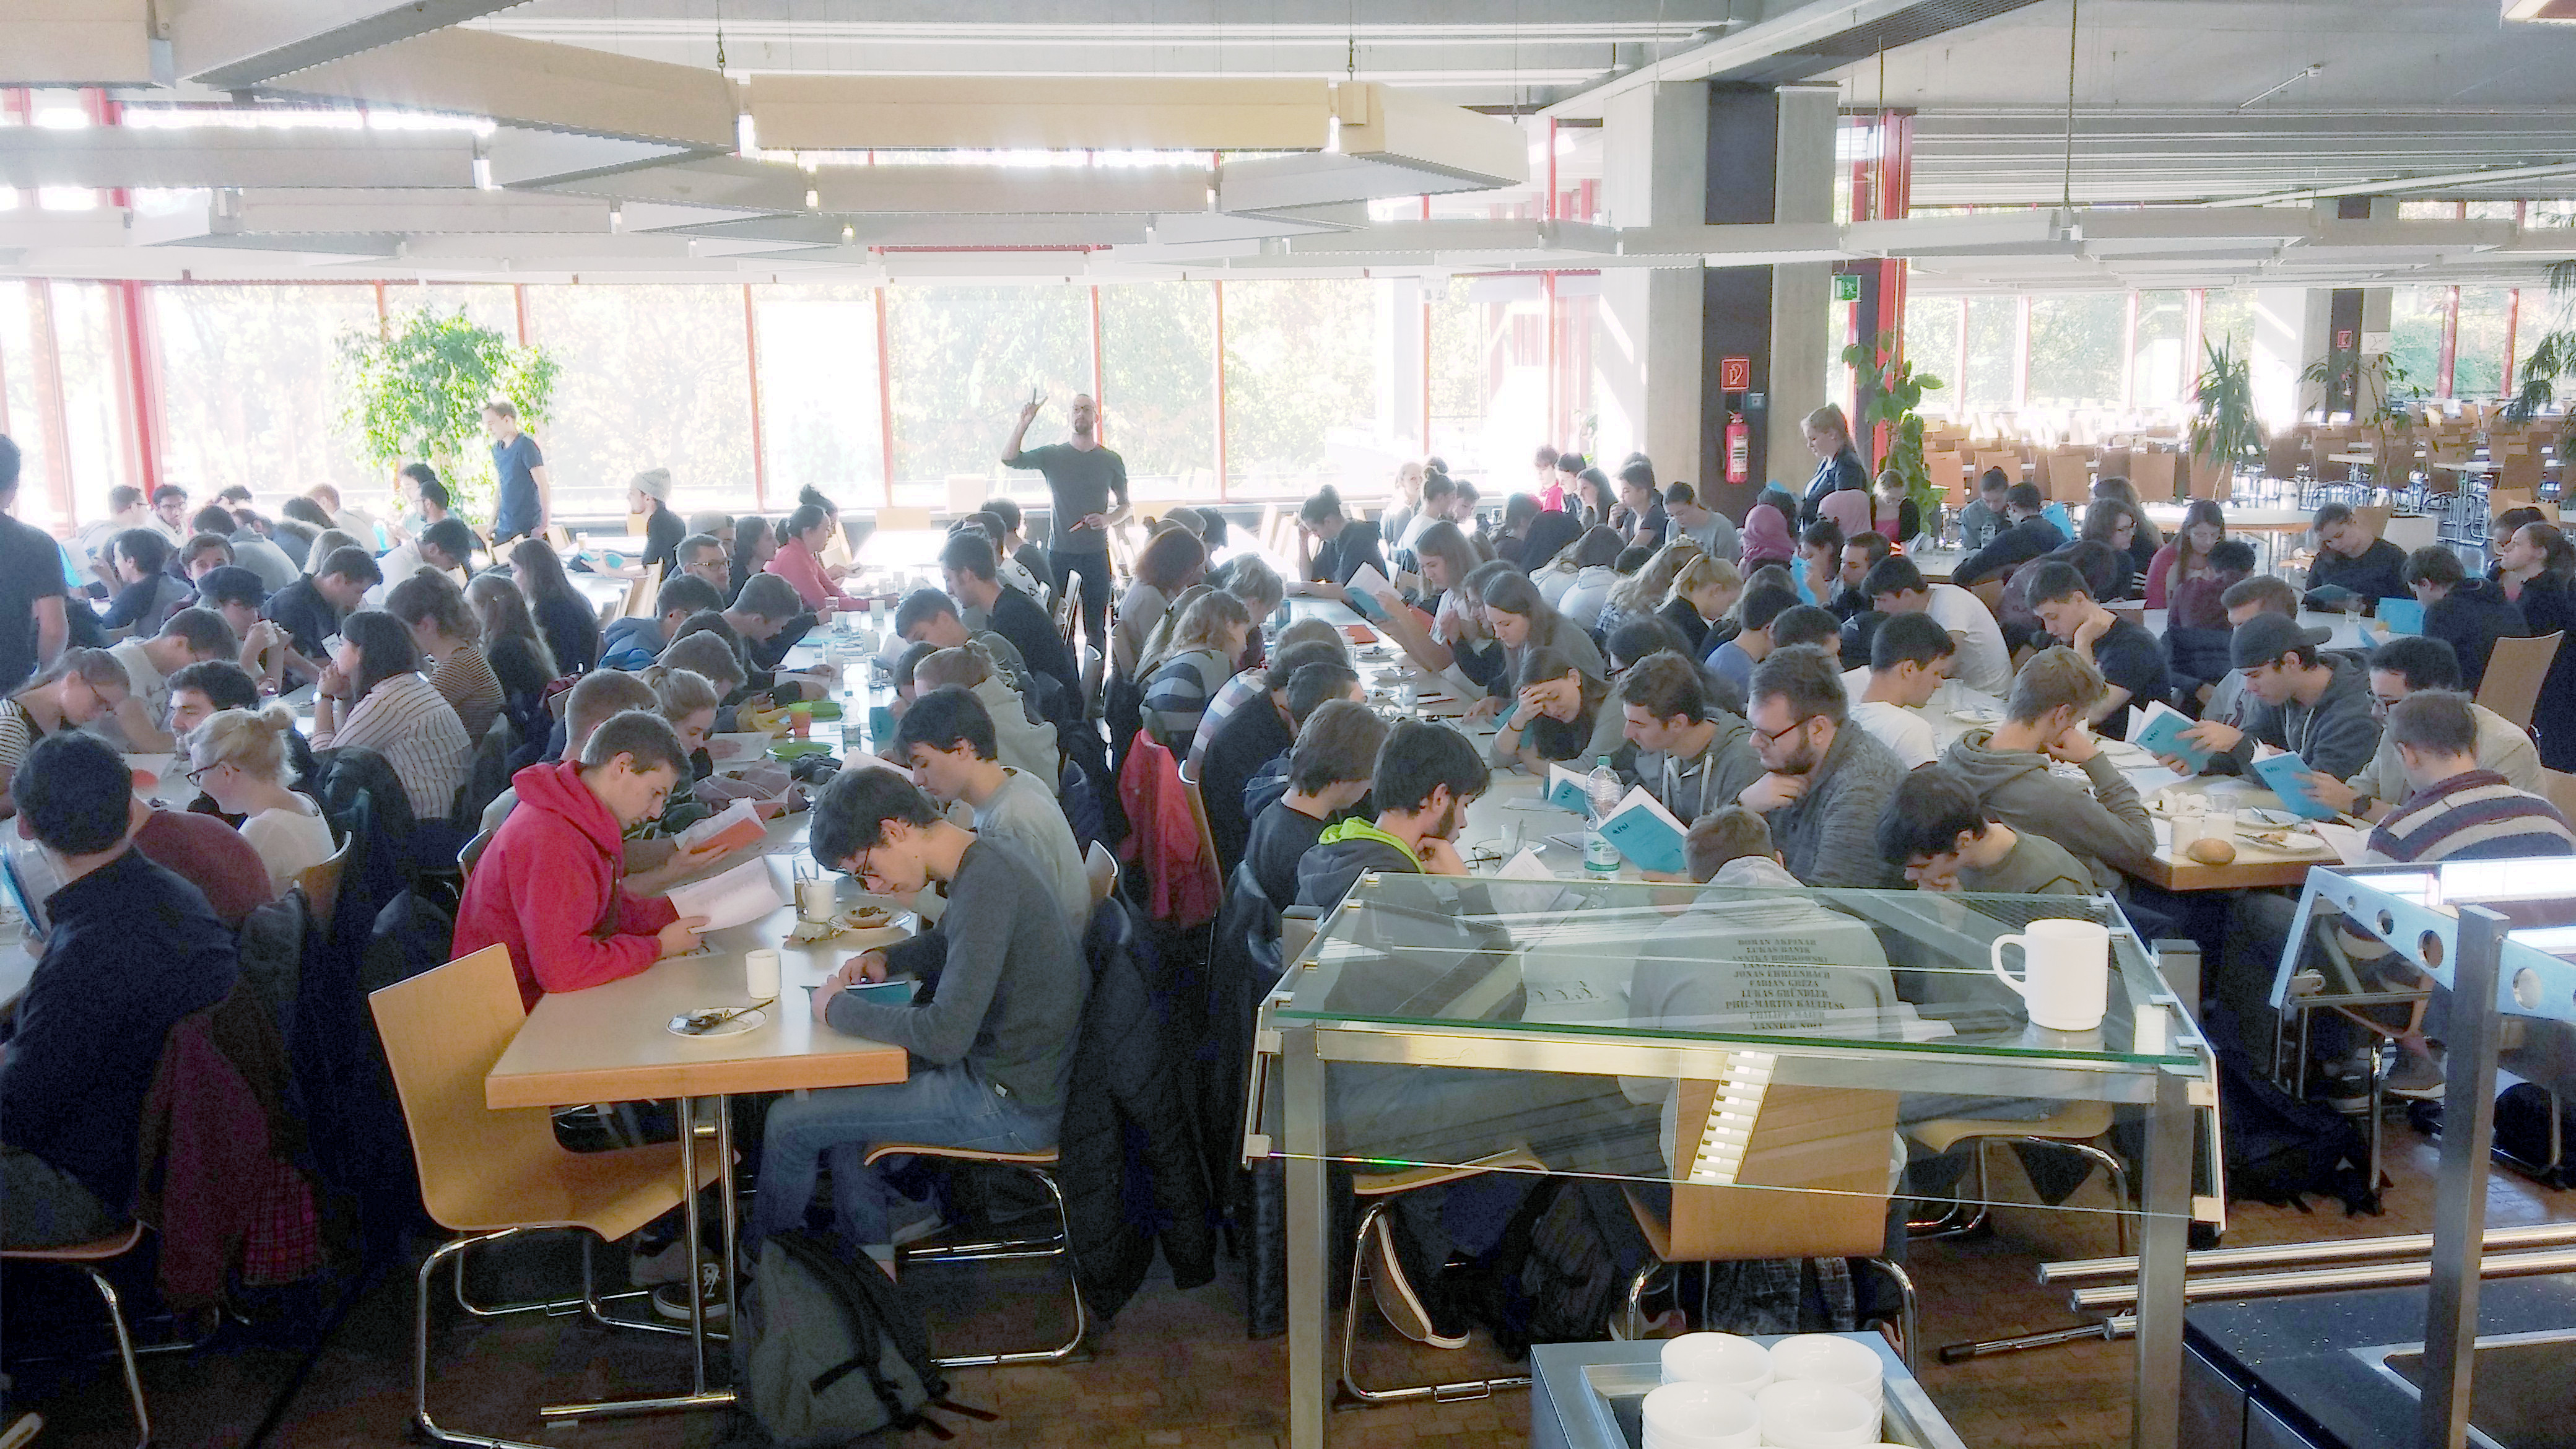
\includegraphics[width=\linewidth]{pictures/fruehstueck_18.jpg}
	\end{columns}
	\end{frame}
	
	\begin{frame}{Anfibrief und Anfiheft}
		\begin{columns}
			\begin{column}{.5\linewidth}
				
\includegraphics[height=0.8\textheight]{pictures/anfibriefe_ws18.png}
			\end{column}
			\begin{column}{.5\linewidth}
				
\includegraphics[height=0.8\textheight]{pictures/anfihefte_ws18.png}
			\end{column}
		\end{columns}
		Auch online: \url{https://www.fsi.uni-tuebingen.de/erstsemester/material/start}
	\end{frame}
	

	\begin{frame}{Partys \& Feste}
		\framesubtitle{ClubHausFest}
		\pause 
		\begin{columns}
			\begin{column}{.6\linewidth}
				\begin{itemize}[<+->]
					\item jeden Donnerstag
					\item im Clubhaus (gegenüber der neuen Aula)
					\item Jede Woche von anderer Fachschaft/Gruppierung
					%\item CHF der Fachschaften Info/Kogni/Psycho am 09.11.
					\item \textbf{Eintritt frei, Studentenausweis mitbringen!}
				\end{itemize}
			\end{column}
			\begin{column}{.4\linewidth}
				%
\includegraphics[width=\linewidth]{pictures/chf_jodel.jpg}
				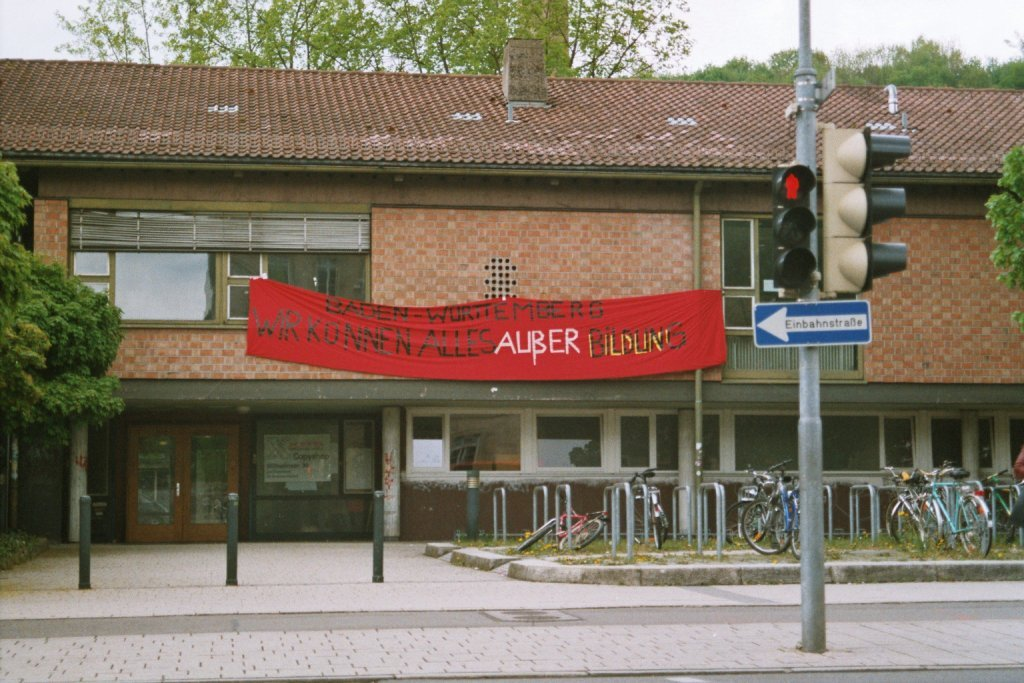
\includegraphics[width=\linewidth]{pictures/clubhaus.jpg} \\
				\footnotesize http://mapio.net/o/2026708/
			\end{column}
		\end{columns}
	\end{frame}

	\begin{frame}{Partys \& Feste}
		\framesubtitle{Sommerfest}
		\pause 
		\begin{figure}
			\centering
			
\includegraphics[height=0.75\textheight]{pictures/sommerfest_18.png}
			%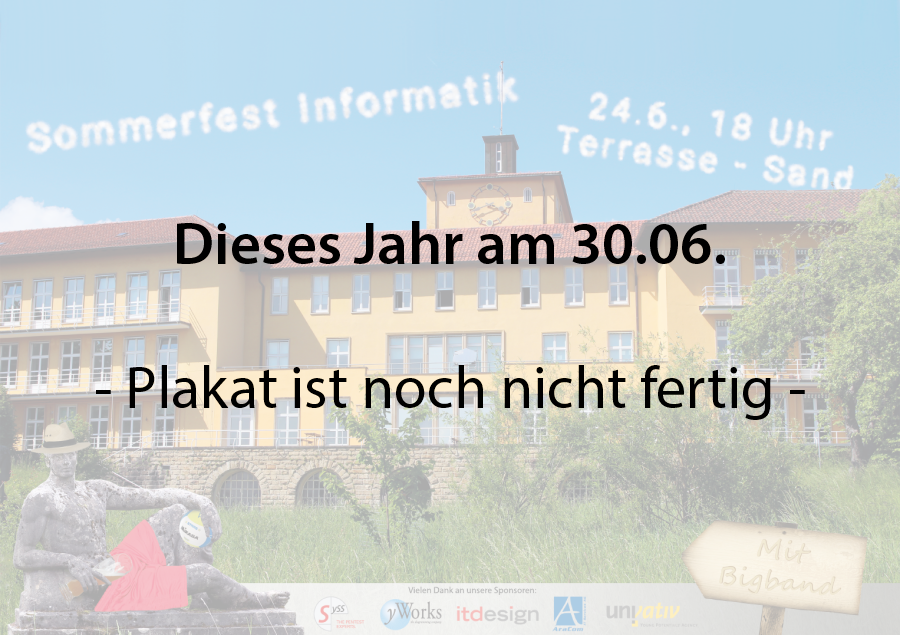
\includegraphics[width=0.9\textwidth]{pictures/sommerfest_platzhalter.png}
		\end{figure}
	\end{frame}
	
	\begin{frame}{Partys \& Feste}
		\framesubtitle{weiteres}
		\pause 
		\begin{itemize}[<+->]
			\item Spieleabende
			\item Stadtralleys 
			\item LAN-Partys
			\item Pizza backen
			\item Anfi-Wochenende
		\end{itemize}
	\end{frame}
	
	%\begin{frame}{Anfi-Wochenende}
	%	\framesubtitle{in Königsheim (bei Albstadt)}
	%	\begin{itemize}[<+->]
	%	\item Findet 1x pro Jahr statt (Für Anfis im Sommer- und Wintersemester)
	%	\item \textbf{10. November bis 12. November}
	%	\item max. Teilnehmerzahl: $\approx$ 38 Personen
	%	\item Kosten pro Person: \EUR{40} (+ Getränke)
	%	\item Weitere Infos und \textbf{Anmeldung} unter \url{https://www.fsi.uni-tuebingen.de/erstsemester/veranstaltungen/wochenende}
	%\end{itemize}
	%\end{frame}
	
%	\begin{frame}{Hochschulpolitik \& Gremien}
%		\framesubtitle{Fakultätsrat}
%	 	Entscheidet über
%	 	\begin{itemize}[<+->]
%	 		\item Finanzen
%	 		\item neue Professuren
%	 		\item Forschung und Lehre
%	 		\item Besetzung von Gremien
%	 	\end{itemize}
%	 	Wird jährlich von allen Studierenden der Fakultät gewählt (5 Studenten aus 11 Fachschaften).
%	 \end{frame}
	
	%\begin{frame}{Hochschulpolitik \& Gremien}
	%	\framesubtitle{Studienkommission}
	% 	\begin{itemize}[<+->]
	% 		\item Wichtigstes Gremium für den Studienablauf
	% 		\item Gestaltet Modulhandbuch
	% 		\item Zwei Kommissionen:
	% 			\begin{itemize}[<+->]
	% 				\item (Bio-, Medien-, Medizin-) Informatik
	% 				\item Kognitionswissenschaft
	% 			\end{itemize}
	% 		\item 4 Profs, 2 Mitarbeiter, 4 Fachschaftler\\
	% 	\end{itemize}
	% \end{frame}
	
%	\begin{frame}{Hochschulpolitik \& Gremien}
%		\framesubtitle{Prüfungsausschuss}
%	 	\begin{itemize}[<+->]
%	 		\item Anerkennung von Studienleistungen
%	 			\begin{itemize}[<+->]
%	 				\item Auslandssemester?
%	 				\item ungewöhnliche Vorlesung für ein bestimmtes Modul?
%	 				\item neues Nebenfach?
%	 			\end{itemize}
%	 		\item (theoretisch) PA für jeden Studiengang einzeln
%	 		\item Fachschaftler mit beratender Stimme
%	 	\end{itemize}
%	 \end{frame}
%	
%	\begin{frame}{Hochschulpolitik \& Gremien}
%		\framesubtitle{weitere studentische Gremien}
%	 	\begin{itemize}[<+->]
%	 		\item StuRa - Studierendenrat (ersetzt AStA)
%	 			\begin{itemize}[<+->]
%	 				\item Hochschulpolitisches Mandat
%	 				\item kann Projekte unterstützen
%	 				\item Gebühren zu Beginn des Semesters
%	 			\end{itemize}
%	 		\item Senat
%	 		\item Vertreter fühlen sich meist einer Hochschulpolitischen Gruppe zugehörig:
%	 			\begin{itemize}[<+->]
%	 				\item FSVV
%	 				\item GHG
%	 				\item JuSos
%	 				\item RCDS
%	 				\item ...
%	 			\end{itemize}
%	 	\end{itemize}
%	 \end{frame}


		\begin{frame}{u.v.a.m.}
			\centering 
			\begin{huge}
				Und noch viel mehr anderen geilen Scheiß!
			\end{huge}
			\vspace*{0.5cm}\\
			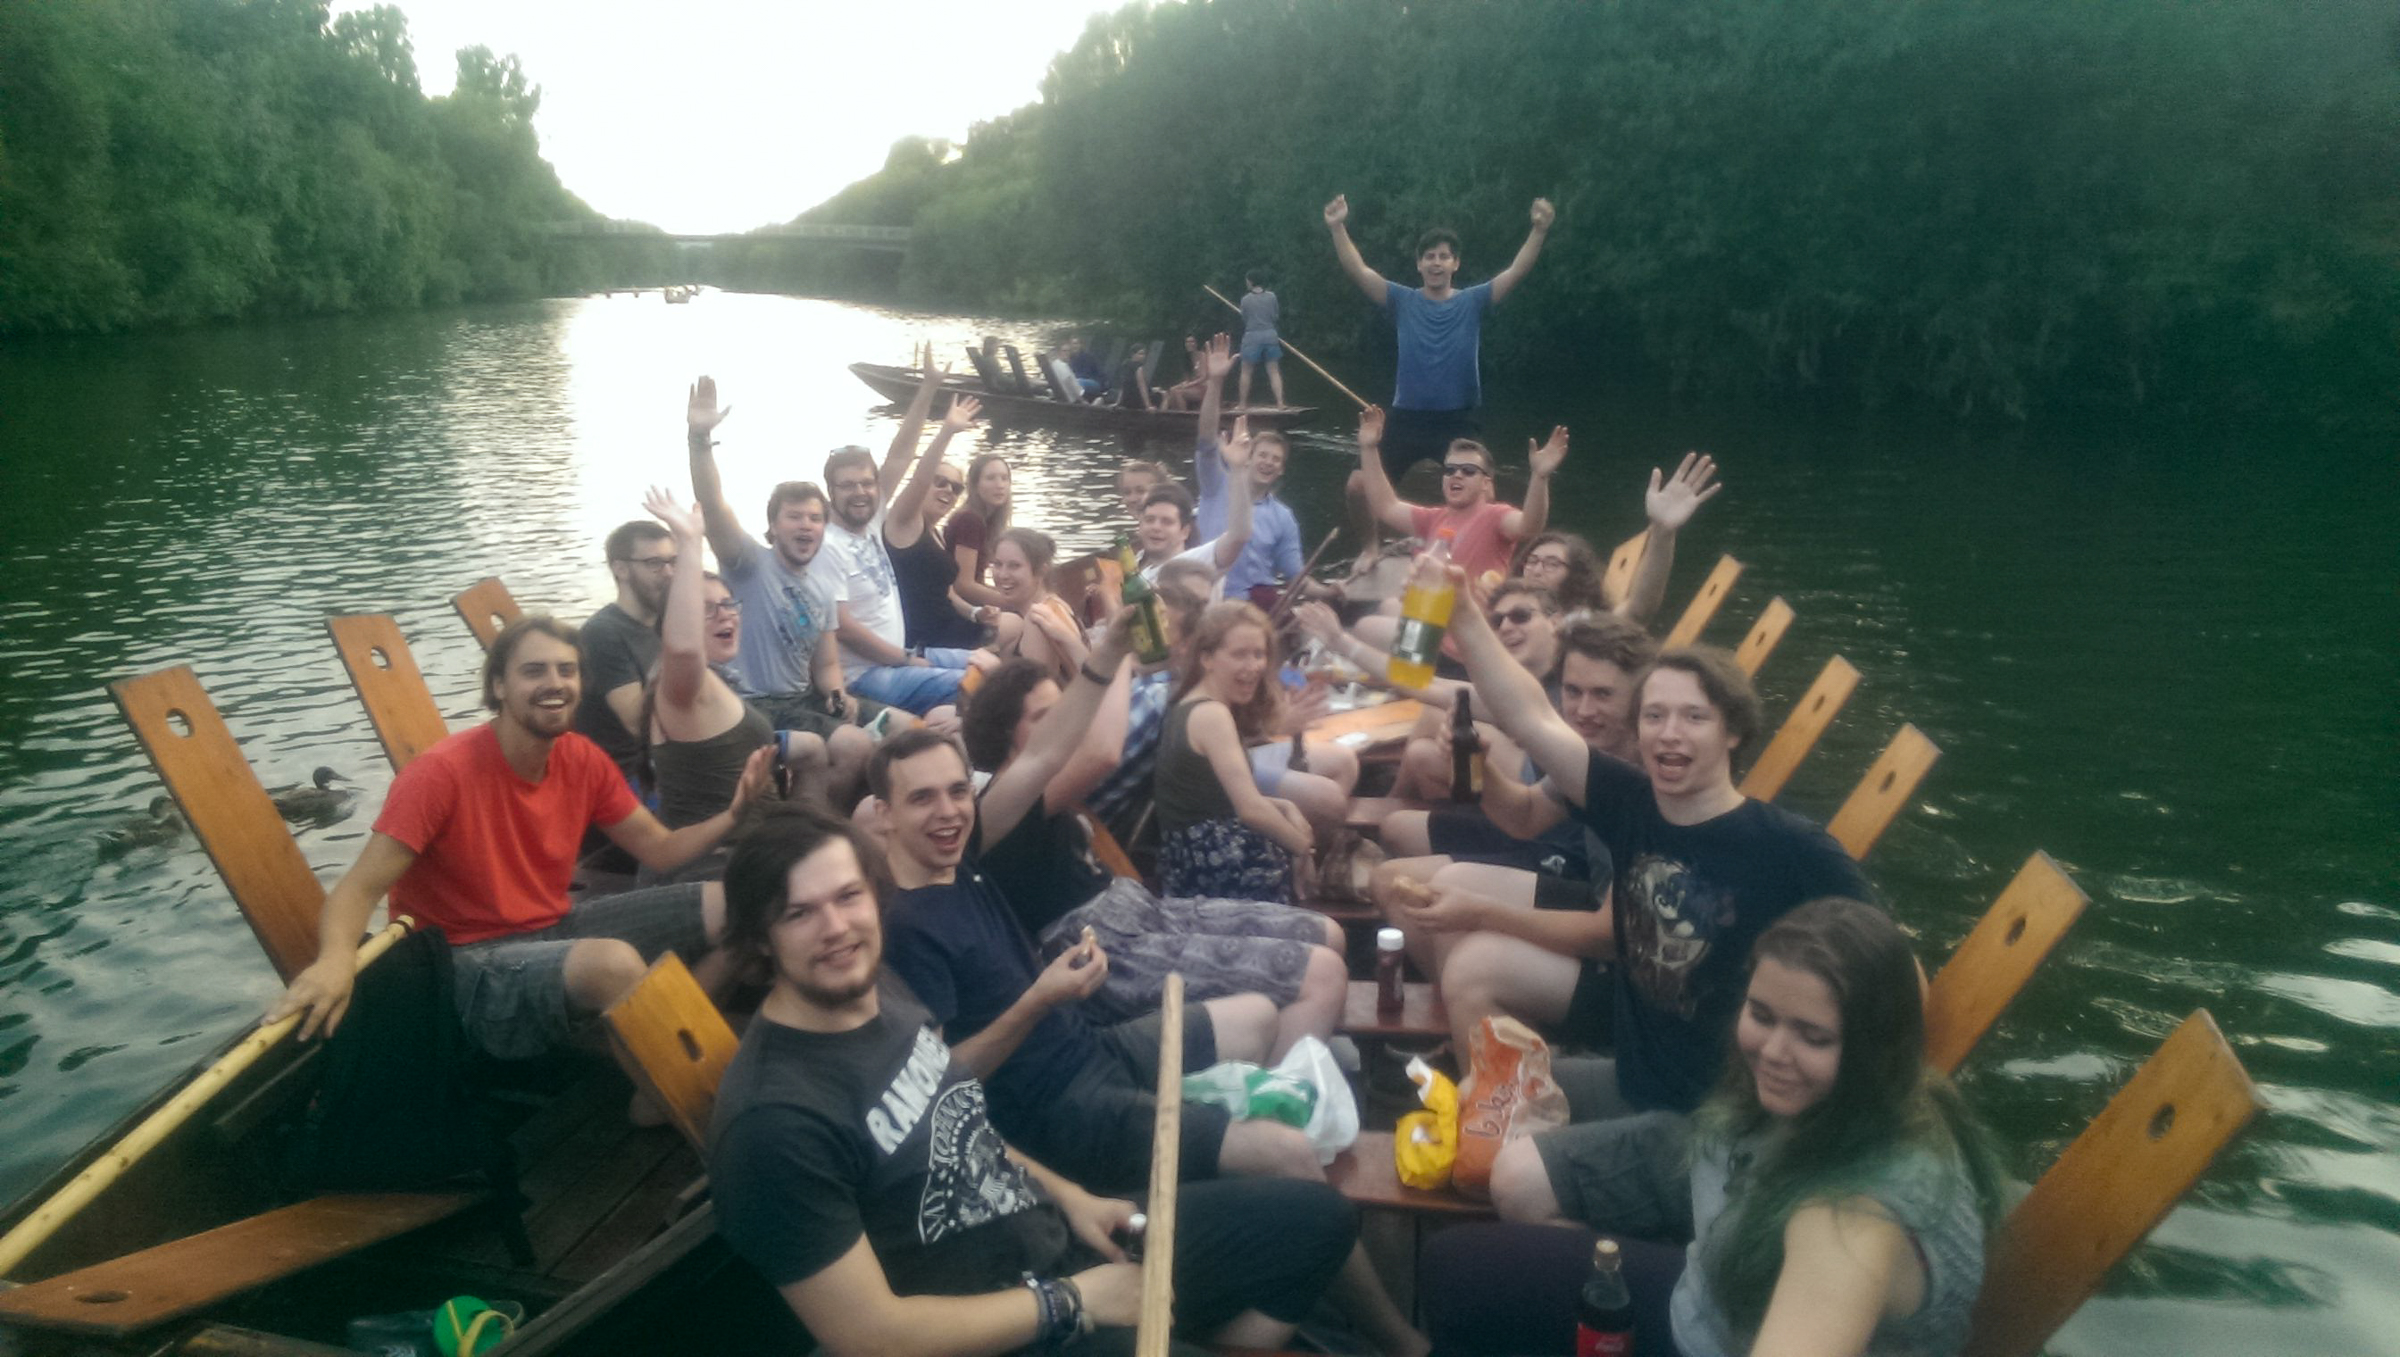
\includegraphics[height=0.6\textheight]{pictures/stocherkahn.jpg}
		\end{frame}
	
	\begin{frame}{Fachschaftsarbeit}
		\framesubtitle{wie geht das?}
		\pause 
		\begin{columns}
			\begin{column}{.5\linewidth}
				\begin{itemize}[<+->]
					\item einfach vorbeikommen und mitmachen ;-)
					\item regelmäßige Treffen im Fachschaftszimmer (Sand, Zimmer C125)
					\item nächstes Treffen: \\Donnerstag 08.11. 18:30 Uhr
					\item teilweise weitere Treffen zu Teilbereichen der Fachschaftsarbeit
					\item Kogni-Treffen: \emph{folgt}
					\item \textbf{Kommt vorbei!}
				\end{itemize}
			\end{column}
			\begin{column}{0.5\linewidth}
				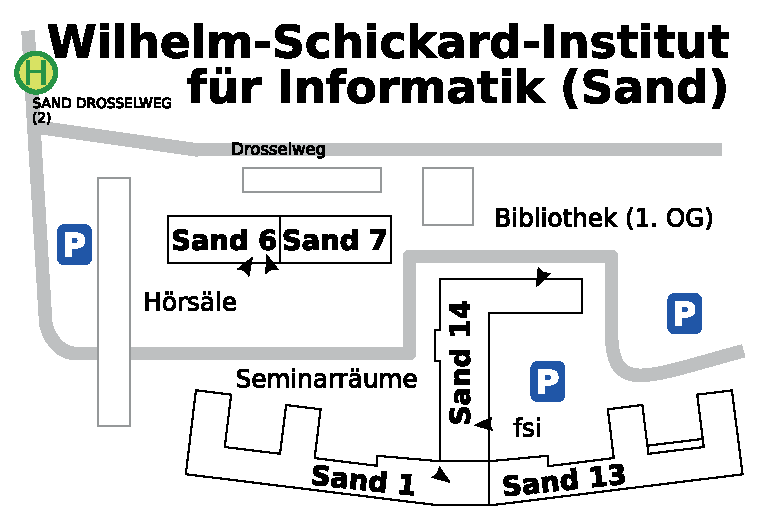
\includegraphics[width=0.7\linewidth]{pictures/uebersicht_sand.pdf}\\
				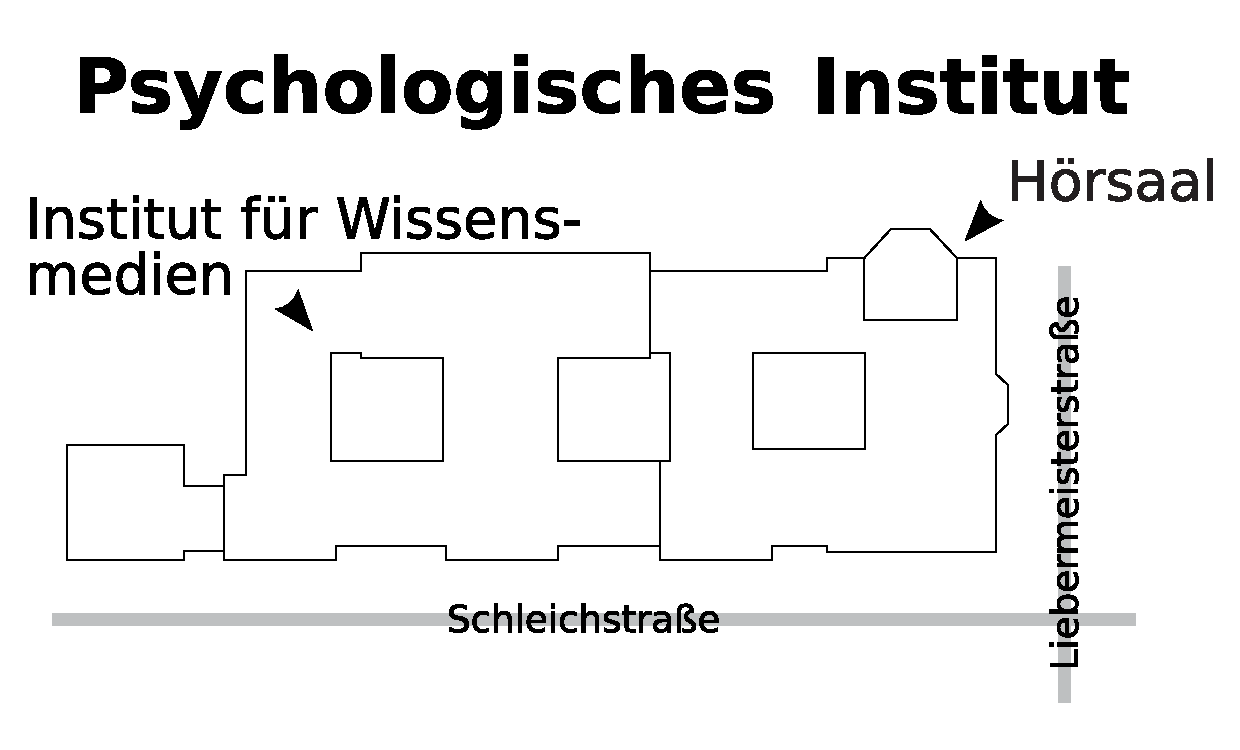
\includegraphics[width=0.7\linewidth]{pictures/uebersicht_pi.pdf}\\
			\end{column}
		\end{columns}
	\end{frame}
	
%	\begin{frame}{Freizeit}
%		\centering 
%		
%	\end{frame}
	
	\begin{frame}
		\begin{columns} 
			\column{0.3\textwidth}
			
\includegraphics[width=\linewidth]{pictures/keepcalm.pdf}
			\column{0.3\textwidth}
			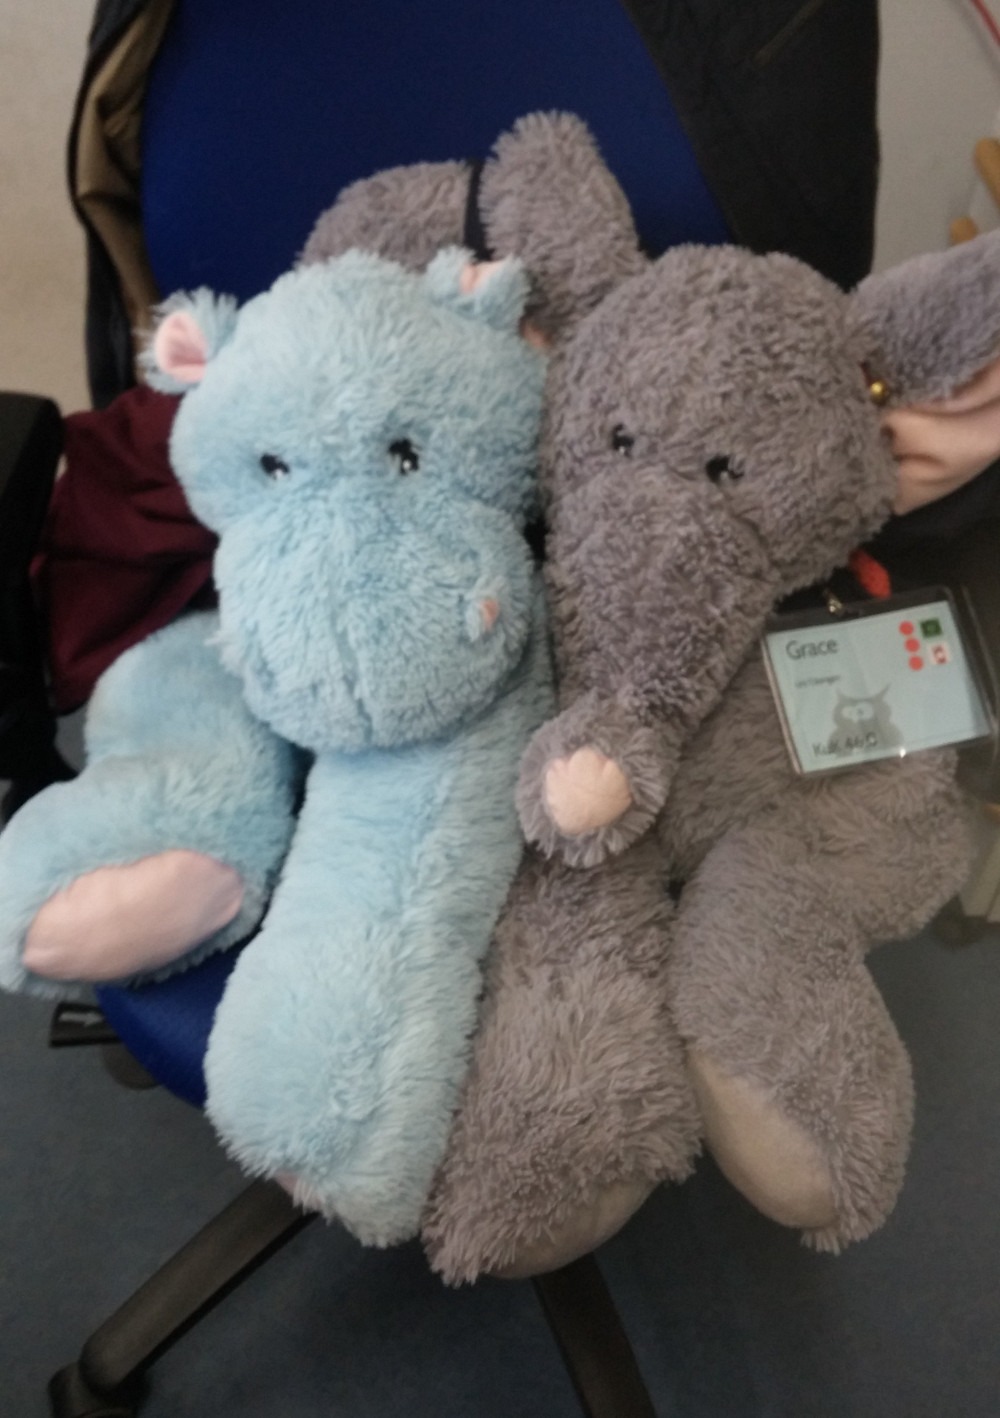
\includegraphics[width=0.9\linewidth]{pictures/grace_siggi.jpg}
			\column{0.4\textwidth}
			\centering
			\begin{huge}
				Wir freuen uns auf euch! \vspace*{1cm}
			\end{huge}
			
			\qrcode{https://www.fsi.uni-tuebingen.de}\\
			\begin{scriptsize}
				\url{https://www.fsi.uni-tuebingen.de}
			\end{scriptsize}
		\end{columns}
		
	\end{frame}

\end{document}
